% !TeX document-id = {678c6d45-9f8c-4926-8cab-e4ae58b13f36}
% !TeX TXS-program:compile = txs:///pdflatex/[--shell-escape]


\documentclass[fleqn,11pt,aspectratio=169]{beamer}
\usepackage{tubslogo}
\usepackage{amsmath}
\usepackage{amsfonts}
\usepackage{amssymb}
\usepackage{graphicx}
\usepackage{geometry}
\usepackage{tikz}
\usepackage{amsthm}
\usepackage{float}
\usepackage{cleveref}
\usepackage{acronym}

\usepackage{fancyvrb}
\usepackage{fvextra}
\usepackage[normalem]{ulem}
\usepackage{enumerate}

\usepackage[overload]{textcase}
\usepackage{minitoc}        
%\usepackage{etoc}        
\usepackage{printlen}
\usepackage{url}  
\usepackage{tabularx}  
\usepackage{soul}
\usepackage{siunitx}
\usepackage{eqparbox}
\sisetup{
	per-mode=symbol,
}
\usepackage[utf8]{inputenc}
\usepackage[
	backend=biber,
	style=numeric,
]{biblatex}

\usepackage[rgb,dvipsnames]{xcolor}

\selectcolormodel{natural}
\usepackage{ninecolors}
\selectcolormodel{rgb}
\usepackage{tabularray}
\usepackage{minted}

\usepackage[export]{adjustbox}% http://ctan.org/pkg/adjustbox

\usepackage[append]{beamersubframe}
\usepackage[american]{babel}
\usepackage{graphicx}
\setbeamerfont{normal text}{size=12pt}

\date{April 23, 2026}
\usetheme[%
  %nexus,%        Nexus Fonts benutzen
  %lnum,%         Versalziffern verwenden
  %cmyk,%<rgbprint>,          Auswahl des Farbmodells
  blue,%<orange/green/violet> Auswahl des Sekundärfarbklangs
  dark,%<light,medium>        Auswahl der Helligkeit
  %colorhead,%    Farbig hinterlegte Kopfleiste
  %colorfoot,%    Farbig hinterlegt Fußleiste auf Titelseite
  colorblocks,%   Blöcke Farbig hinterlegen
  %nopagenum,%    Keine Seitennumer in Fußzeile
  %nodate,%       Kein Datum in Fußleiste
  tocinheader,%   Inhaltsverzeichnis in Kopfleiste
  %tinytocinheader,% kleines Kopfleisten-Inhaltsverzeichnis
  %widetoc,%      breites Kopfleisten-Inhaltsverzeichnis
  %narrowtoc,%    schmales Kopfleisten-Inhaltsverzeichnis
  %nosubsectionsinheader,%  Keine subsections im Kopfleisten-Inhaltsverzeichnis
  %nologoinfoot,% Kein Logo im Fußbereich darstellen
  ]{tubs}
% Titelseite
%\title{towards TPU: A Survey into Accelerators for Cloud AI}
\title{Algorithm Engineering 2026: Sheet 01}
\author{Rouven Kniep}

%titlepage font and background
\setbeamercolor{titlebarfirst}{parent=titlepage, bg=titlepage.bg!0}

% Edit the TUBS template to move the tubslogo into place for the title
\let\tubslogoAbsOld\tubslogoAbs
\renewcommand{\tubslogoAbs}[1]{\raisebox{6.877mm}{\tubslogoAbsOld{#1}}}

% Quoteblock 
\newcommand{\quotebox}[1]{\begin{center}\fcolorbox{white}{blue!15!gray!15}{\begin{minipage}{0.9\linewidth}\vspace{10pt}\center\begin{minipage}{0.8\linewidth}{\space\Huge``}{#1}{\hspace{1.5em}\break\null\Huge\hfill''}\end{minipage}\smallbreak\end{minipage}}\end{center}}



\newcommand<>{\overlay}[1]{\only#2{%
		\AddToHookNext{shipout/foreground}{%
			\begin{tikzpicture}[remember picture,overlay]%
				\draw[fill=black,opacity=0.70] 
				(current page.north east) rectangle (current page.south west);
				\node at (current page.center) {#1};
	\end{tikzpicture}}}
}


\begin{document}

\part{main}
\begin{frame}[plain]
	\titlepage
\end{frame}	

% Edit the TUBS template to move the tubslogo into place for the footer
\renewcommand{\tubslogoAbs}[1]{\raisebox{-6.2pt}{\tubslogoAbsOld{#1}}}
\newlength{\fw}
\setlength{\fw}{7pt}

% make all verbatims to block verbatims
\RecustomVerbatimEnvironment{Verbatim}{BVerbatim}{}

\section{Producer-Consumer}

\begin{frame}{Consumer Producer}
\begin{itemize}
	\item Scenario: 60 Producers, 1 Consumer 
	\item Production rate: 1 per 2 weeks
	\item Consumption rate: 1 per 20-30 minutes
	\item $\implies$ Consumer Workload: ~60 hours/month
	\item $\implies$ Consumer Overload!	
\end{itemize}
\end{frame}

\begin{frame}{Consumer Producer (alternative)}
	\begin{itemize}
		\item Scenario: 60 Producers, 1 Consumer 
		\item \textbf{Optimization: pair producers}
		\item Production rate: 1 per 2 weeks
		\item Consumption rate: 1 per 20-30 minutes
		\item $\implies$ Consumer Workload: \textbf{~30 hours/month}
		\item $\implies$ \textbf{Consumer happy!}	
		\item $\implies$ \textbf{Producers practice collaboration}
	\end{itemize}
\end{frame}

\begin{frame}[important]{In other news......}
	
	\begin{center}
		\fbox{
			\parbox{\textwidth}{
				\centering\begin{tblr}{c}
					\textbf{\large }\\
					\textbf{\huge GROUP UP!}\\
					\textbf{\large or i'll do it}\\
					\textbf{Email me with your partner before sunday night.}\\
					\textbf{Otherwise: Skill-based matchmaking.}
				\end{tblr}
			}
		}
	\end{center}
\end{frame}
	

\section{Ex2: Bad Programs}

\begin{frame}{Branch Prediction: correct prediction}
	\texttt{\begin{tblr}{colspec={r|c|ccccccccc}, column{5}={GreenYellow}}
		PC & instruction & \SetCell[c=9]{} Cycle 1, 2, ... &&&&&&&	&	\\
		\hline
		0x20 & add r3 = r2+r1 		&IF	&ID	&EX	&M	&WB	&	&	&	&	\\
		0x24 & bge r3 >= r4, 0x8 	& 	&IF &ID	&EX &M	&WB &	&	&	\\
		0x32 & load r5[r3] 			&	& 	&IF &ID	&EX & M	&WB &	&	\\
		0x36 & load r6[r1] 			&	&	& 	&IF &ID	&EX & M	&WB &	\\ 
		0x40 & call turn() 			&	&	&	& 	&IF &ID	&EX & M	& WB\\
	\end{tblr}}
	\begin{center}
		branch correctly predicted, no penalty
	\end{center}
\end{frame}


\begin{frame}{Branch Prediction: misprediction penalty}
	\texttt{\begin{tblr}{colspec={r|c|ccccccccccc}, column{5}={Lavender}, column{7}={GreenYellow}}			
			\hline
			PC & instruction & \SetCell[c=10]{} Cycle 1, 2, ... &&&&&&&	&	&	&	\\
			0x20 & add r3 = r2+r1 		&IF	&ID	&EX	&M	&WB	&	&	&	&	&	&	\\
			0x24 & blt r3 < r4, 0x8 	& 	&IF &ID	&EX &M	&WB &	&	&	&	&	\\
			0x28 & sub r3 = r3 - r4		&   &   &IF &ID &-- &	&	&	&	&	&	\\
			0x32 & load r5[r3] 			&	& 	&	&IF &--	& 	&	&	&	&	&	\\
			0x32 & load r5[r3] 			&	& 	&	&	&IF &ID	&EX & M	&WB &	&	\\
			0x36 & load r6[r1] 			&	&	&	&	& 	&IF &ID	&EX & M	&WB &	\\ 
			0x40 & call turn() 			&	&	&	&	&	& 	&IF &ID	&EX & M	&WB	\\
	\end{tblr}}
	\begin{center}
		misprediction! first wrong instruction in \textcolor{Lavender}{Cycle 3}, correct in \textcolor{GreenYellow}{Cycle 5} $\implies$ 2 cycles penalty
		Real CPUs: AMD Zen4 $\approx$13; Intel Lion Cove $\approx$14; ARM Oryon $\approx$13; \dots  \
	\end{center}
\end{frame}

\begin{frame}[fragile]{CMOV in assembly}
	\centering\texttt{cmovae r3, r4} = overwrite \texttt{r3} with \texttt{r4} if "above or equal" flag is set
	\vspace{20pt}
	
	\begin{columns}
		\column{0.4\textwidth}
		without CMOV: branch!
		
		\vspace{4pt}
		
		\begin{BVerbatim}[breaklines=true,commandchars=\\\{\}, tabsize=4]
0x20: add r3 = r2+r1
0x24: blt r3 < r4, +0x8
0x28: sub r3 = r3-r4
0x32: load r5[r3]
		\end{BVerbatim}
		
		\column{0.4\textwidth}
		with CMOV: branchless
		
		\vspace{4pt}
		
		\begin{BVerbatim}[breaklines=true,commandchars=\\\{\}, tabsize=4]
0x20: add r3 = r2+r1
0x24: sub r4 = r3-r4
0x28: cmovae r3, r4,
0x32: load r5[r3]
		\end{BVerbatim}
	\end{columns}
\end{frame}

\begin{frame}[fragile]{2a: Branch Misses}
	\begin{center}	
		\begin{minted}[tabsize=2]{c++}
std::size_t ax = i + j;
if(i + j >= n) {
	ax -= n;
}
std::int64_t a_i = a[ax];
std::int64_t b_j = b[j];
auto t1 = turn({x, y}, {a_i, b_j}, {b_j, a_i});
if(t1 >= 0) {
	auto t2 = turn({x, y}, {-b_j, -a_i}, {-a_i, -b_j});
	if(t2 >= 0) {
		result += c[(a_i + b_j) % m] * (t1 + t2 + 1);
	}
}
		\end{minted}
	\end{center}
\end{frame}


\begin{frame}[fragile]{2a: State (dirty data)}
	\begin{center}	
		\texttt{sudo perf stat ./Release/problem\_program\_a 16384}
		
		\vspace{10pt}
		
		\begin{minted}[tabsize=2]{text}
 8.944.560.992      cpu_atom/instructions/           #    1,52  insn per cycle              (0,24%)
25.285.677.974      cpu_core/instructions/           #    1,64  insn per cycle              (99,71%)
 1.165.887.659      cpu_atom/branches/               #  285,789 M/sec                       (0,24%)
 2.868.382.421      cpu_core/branches/               #  703,113 M/sec                       (99,71%)
    69.752.046      cpu_atom/branch-misses/          #    5,98% of all branches             (0,26%)
   272.508.200      cpu_core/branch-misses/          #    9,50% of all branches             (99,71%)
		\end{minted}
		
		\vspace{10pt}
		\dots but inconsistent! why? - multiple core types and switching between them
	\end{center}
\end{frame}

\begin{frame}[fragile]{2a: State}
	\begin{center}	
		\texttt{taskset -c 1 sudo perf stat ./Release/problem\_program\_a 16384}
		
		\vspace{10pt}
		
		\begin{minted}[tabsize=2]{text}    
25.215.879.289      cpu_core/instructions/           #    1,61  insn per cycle
 2.859.518.614      cpu_core/branches/               #  838,477 M/sec                     
   271.903.112      cpu_core/branch-misses/          #    9,51% of all branches           
		\end{minted}
		
		\vspace{10pt}

	\end{center}
\end{frame}
	

\begin{frame}[fragile]{2a: first if is a CMOV}
	\begin{center}	
		\begin{minted}[tabsize=2]{text}
64	            std::size_t ax = i + j;
65	            if(i + j >= n) {
	0x15f0 <+80>:	4c 39 ef           	cmp    %r13,%rdi
	0x15f3 <+83>:	48 8d 04 1e        	lea    (%rsi,%rbx,1),%rax
	
69	            std::int64_t b_j = b[j];
	0x15f7 <+87>:	4d 8b 14 f4        	mov    (%r12,%rsi,8),%r10
	
66	                ax -= n;
	0x15fb <+91>:	48 0f 42 c7        	cmovb  %rdi,%rax
		\end{minted}
	\end{center}
\end{frame}


\begin{frame}[fragile]{2a: nested if.. [1]}
	\begin{columns}[T]
		\column{0.7\textwidth}
		\begin{minted}[tabsize=2]{c++}
auto t1 = turn({x, y}, {a_i, b_j}, {b_j, a_i});
if(t1 >= 0) {
	auto t2 = turn({x, y}, {-b_j, -a_i}, {-a_i, -b_j});
	if(t2 >= 0) {
		result += c[(a_i + b_j) % m] * (t1 + t2 + 1);
}}
		\end{minted}

		\vspace{10pt}
			
		\begin{columns}
			\column{0.2\textwidth}
			\begin{tblr}{colspec={rl}, colsep=2pt, rowsep=1pt}
				1.25 & seconds \\
				2.86B & branches \\
				271M & \SetCell[r=2]{} misses \\
				9.50\% & \\
			\end{tblr}
			\column{0.5\textwidth}
		\end{columns}
	\end{columns}
\end{frame}


\begin{frame}[fragile]{2a: nested if.. [2]}
	\begin{columns}[T]
		\column{0.7\textwidth}
		\begin{minted}[tabsize=2]{c++}
auto t1 = turn({x, y}, {a_i, b_j}, {b_j, a_i});
auto t2 = turn({x, y}, {-b_j, -a_i}, {-a_i, -b_j});
if(t1 >= 0 && t2 >= 0) {
	result += c[(a_i + b_j) % m] * (t1 + t2 + 1);
}
		\end{minted}
		
		\vspace{10pt}
		
		\begin{columns}
			\column{0.2\textwidth}
			\begin{tblr}{colspec={rl}, colsep=2pt, rowsep=1pt}
				0.35 & seconds \\
				2.72B & branches \\
				137M & \SetCell[r=2]{} misses \\
				5.04\% & \\
			\end{tblr}
			\column{0.6\textwidth}
			\begin{itemize}
				\item idea: second turn "cheap"\\
					(4 Sub + 2 Mul + no loads)
				\item compiler cannot safely move calls
			\end{itemize}
		\end{columns}
	\end{columns}
\end{frame}

\begin{frame}[fragile]{2a: nested if..? [3]}
	\begin{columns}[T]
		\column{0.7\textwidth}
		\begin{minted}[tabsize=2]{c++}
auto t1 = turn({x, y}, {a_i, b_j}, {b_j, a_i});
auto t2 = turn({x, y}, {-b_j, -a_i}, {-a_i, -b_j});
if((t1 | t2) & std::numeric_limits<std::int64_t>::min()) {
	continue;
}
result += c[(a_i + b_j) % m] * (t1 + t2 + 1);    
		\end{minted}
		
		\vspace{10pt}
		
		\begin{columns}
			\column{0.2\textwidth}
			\begin{tblr}{colspec={rl}, colsep=2pt, rowsep=1pt}
				0.35 & seconds \\
				2.72B & branches \\
				137M & \SetCell[r=2]{} misses \\
				5.04\% & \\
			\end{tblr}
			\column{0.5\textwidth}
			\begin{itemize}
				\item help compiler with if-merge => not required
				\item last branch: predictable \\
					(take-rate 2.86e-06)
			\end{itemize}
		\end{columns}
	\end{columns}
\end{frame}

\begin{frame}[fragile]{2a: function calls? [3]}
\begin{columns}[T]
	\column{0.7\textwidth}
	\begin{minted}[tabsize=2]{c++}
inline std::int64_t turn(std::array<std::int64_t, 2> p1,
                         std::array<std::int64_t, 2> p2,
                         std::array<std::int64_t, 2> p3) {
	return (p2[0] - p1[0]) * (p3[1] - p1[1]) - 
	(p2[1] - p1[1]) * (p3[0] - p1[0]);
}
	\end{minted}
	
	\vspace{10pt}
	
	\begin{columns}
		\column{0.2\textwidth}
		\begin{tblr}{colspec={rl}, colsep=2pt, rowsep=1pt}
			0.35 & seconds \\
			2.72B & branches \\
			137M & \SetCell[r=2]{} misses \\
			5.04\% & \\
		\end{tblr}
		\column{0.5\textwidth}
		\begin{itemize}
			\item "force-inline" function
			\item annoying to debug, slower to compile, larger binary
			\item $\implies$ dirty "fix"
			\item \dots but effective
		\end{itemize}
	\end{columns}
\end{columns}
\end{frame}

\begin{frame}[fragile]{2b: data structures [1] - extensions}
	\begin{center}
		\begin{tblr}{c| rrrr}
			candidates & \texttt{set} & \texttt{vector} & \texttt{vector<bool>} & \texttt{vector} \\
			graph 		& adj. list 	& adj. list & 	adj. matrix & adj.matrix\\
					\hline
			graph1 & \qty{0.15}{\second} & \qty{0.09}{\second} & \qty{0.13}{\second} & $\leq$\qty{0.01}{\second}\\
			graph2 & \qty{0.17}{\second} & \qty{0.10}{\second} & \qty{0.14}{\second} & $\leq$\qty{0.01}{\second}\\
			graph3 & \qty{0.28}{\second} & \qty{0.13}{\second} & \qty{0.12}{\second} & $\leq$\qty{0.01}{\second}\\
			graph4 & \qty{0.44}{\second} & \qty{0.19}{\second} & \qty{0.11}{\second} & \qty{0.01}{\second}\\
			graph5 & \qty{0.82}{\second} & \qty{0.15}{\second} & \qty{0.12}{\second} & \qty{0.04}{\second}\\
			graph6 & \qty{1.76}{\second} & \qty{0.84}{\second} & \qty{0.12}{\second} & \qty{0.12}{\second}\\
			graph7 & \qty{2.43}{\second} & \qty{1.25}{\second} & \qty{0.12}{\second} & \qty{0.20}{\second}\\
			graph8 & \qty{5.30}{\second} & \qty{2.90}{\second} & \qty{0.12}{\second} & \qty{0.35}{\second}\\
			graph9 & \qty{4.62}{\second} & \qty{3.02}{\second} & \qty{1.40}{\second} & \qty{0.11}{\second}\\
		\end{tblr}
	\end{center}
\end{frame}


\section{Ex3: Twoopt + Analysis}


\begin{frame}[fragile]{3: twoopt + analysis}
	\begin{columns}[T]
		\column{0.6\textwidth}
		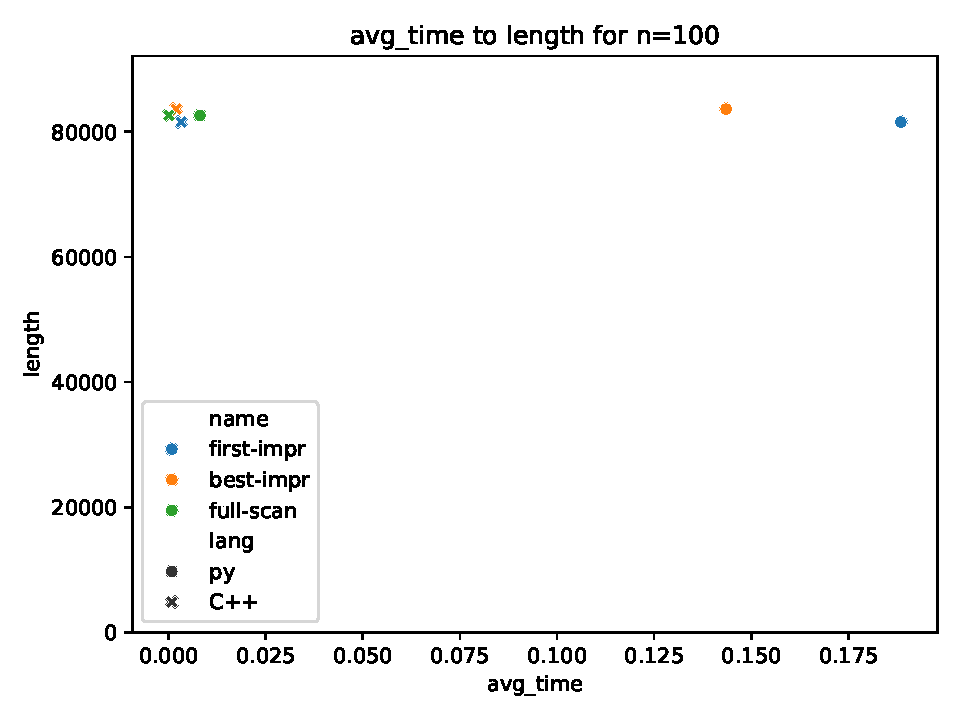
\includegraphics[keepaspectratio, height=0.9\textheight]{3_n100_time_length.pdf}
		
		\column{0.4\textwidth}
		\begin{itemize}
			\item python MUCH slower
			\item full-scan: fastest
			\item first-impr: best\\ BUT slowest!
		\end{itemize}
	\end{columns}
\end{frame}

\begin{frame}[fragile]{3: twoopt + analysis}
\begin{columns}[T]
	\column{0.6\textwidth}
	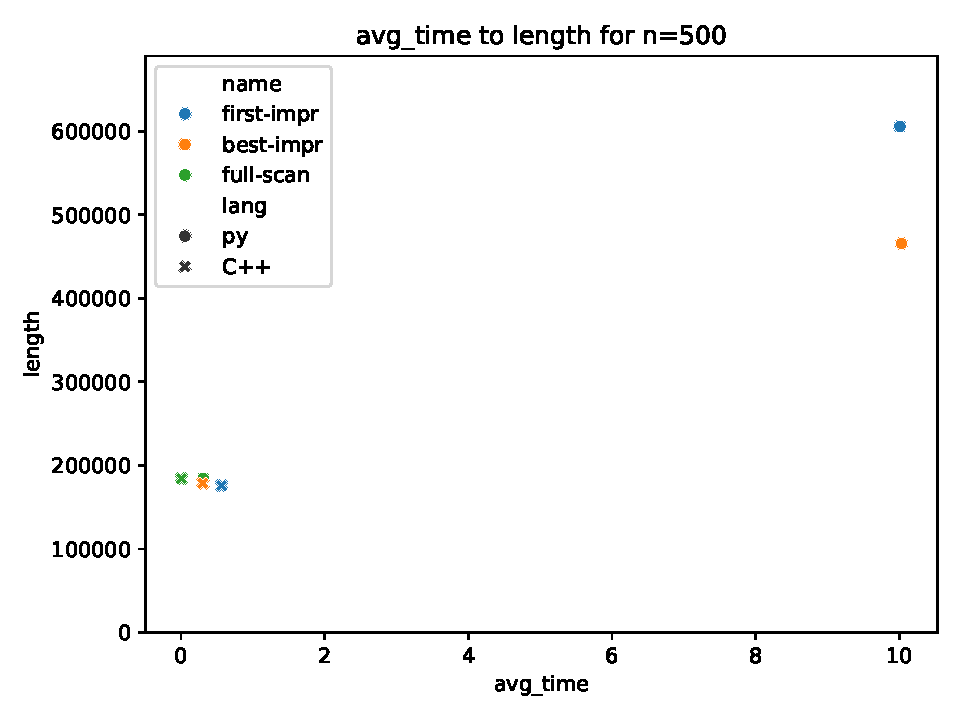
\includegraphics[keepaspectratio, height=0.9\textheight]{3_n500_time_length.pdf}
	
	\column{0.4\textwidth}
	\begin{itemize}
		\item python MUCH slower
		\item full-scan: fastest
		\item first-impr: best\\ BUT slowest!
		\item timeout = horrible
	\end{itemize}
\end{columns}
\end{frame}

\begin{frame}[fragile]{3: twoopt + analysis}
\begin{columns}[T]
	\column{0.6\textwidth}
	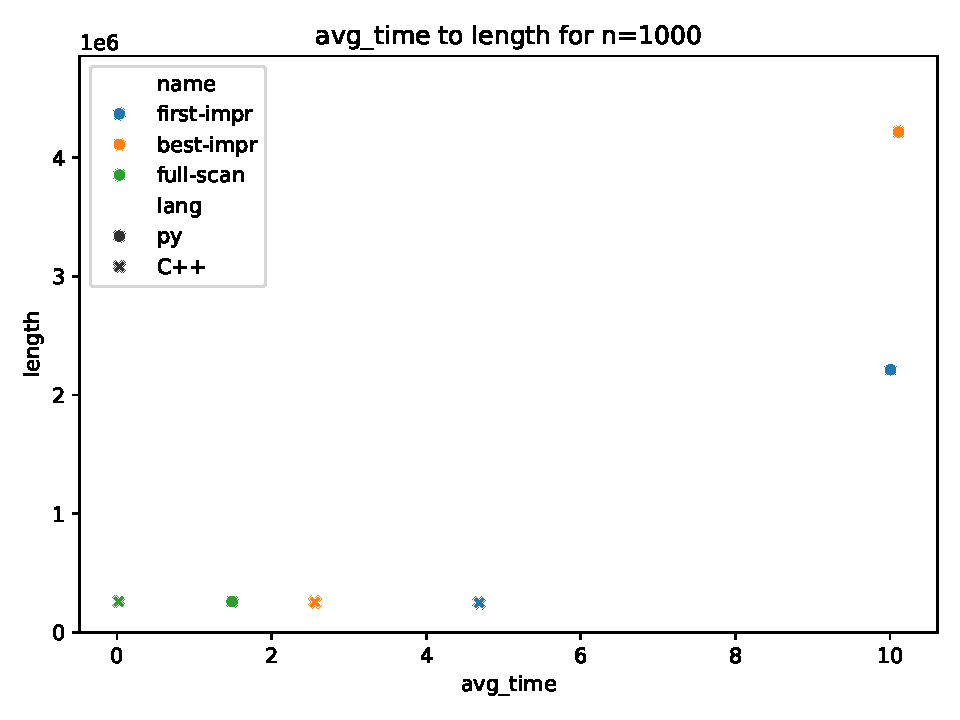
\includegraphics[keepaspectratio, height=0.9\textheight]{3_n1000_time_length.pdf}
	
	\column{0.4\textwidth}
	\begin{itemize}
		\item python MUCH slower
		\item full-scan: fastest \\ by a LOT
		\item first-impr: best\\ BUT slowest!
		\item timeout = horrible
	\end{itemize}
\end{columns}
\end{frame}

\begin{frame}[fragile]{3: twoopt + analysis}
\begin{columns}[T]
	\column{0.6\textwidth}
	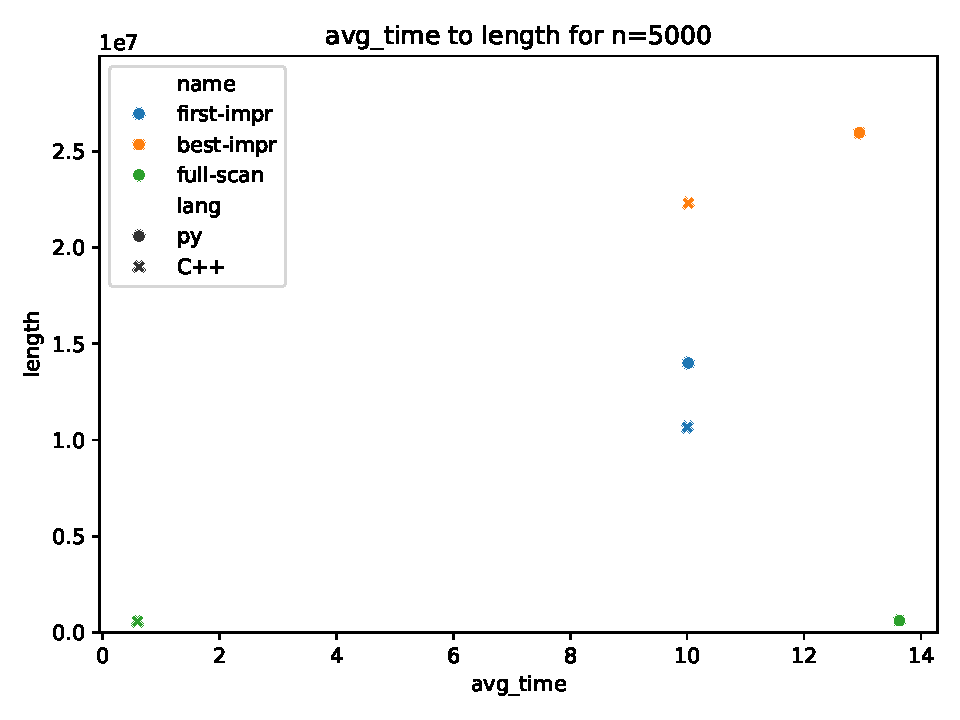
\includegraphics[keepaspectratio, height=0.9\textheight]{3_n5000_time_length.pdf}
	
	\column{0.4\textwidth}
	\begin{itemize}
		\item python MUCH slower
		\item full-scan: fastest \\ by a LOT
		\item first-impr: best\\ BUT slowest!
		\item timeout = horrible
	\end{itemize}
\end{columns}
\end{frame}

\begin{frame}[fragile]{3: twoopt + analysis}
\begin{columns}[T]
	\column{0.6\textwidth}
	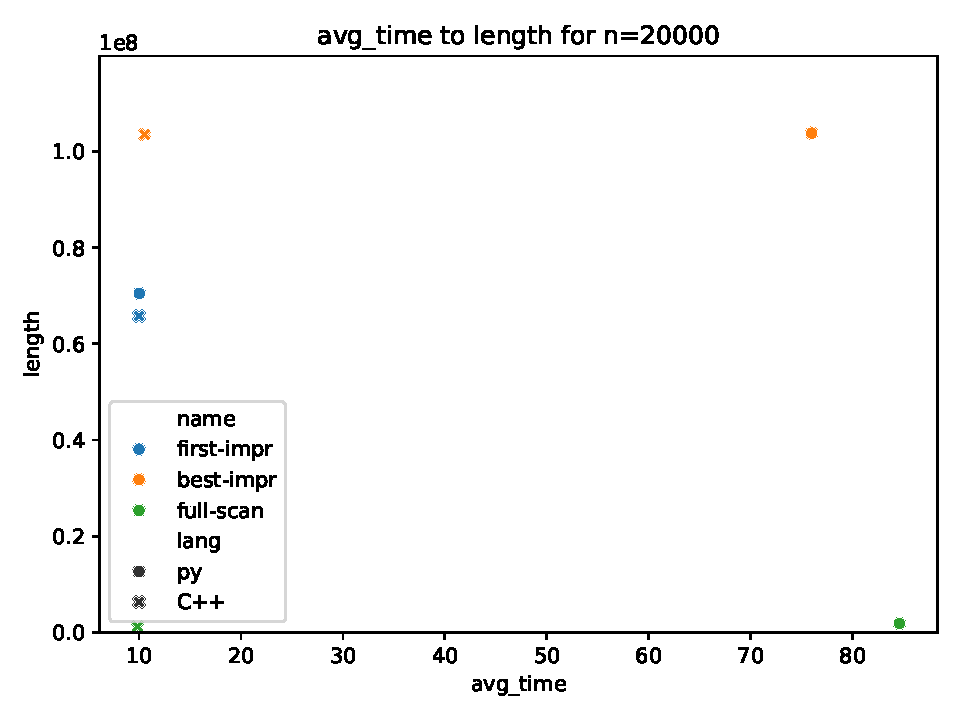
\includegraphics[keepaspectratio, height=0.9\textheight]{3_n20000_time_length.pdf}
	
	\column{0.4\textwidth}
	\begin{itemize}
		\item python MUCH slower
		\item full-scan: fastest \\ by a LOT
		\item first-impr: best\\ BUT slowest!
		\item timeout = horrible
		\item insufficient timeout on python fullscan + python best-impr
	\end{itemize}
\end{columns}
\end{frame}

\begin{frame}[fragile]{3: twoopt + analysis [2]}
	\begin{columns}[T]
		\column{0.6\textwidth}
		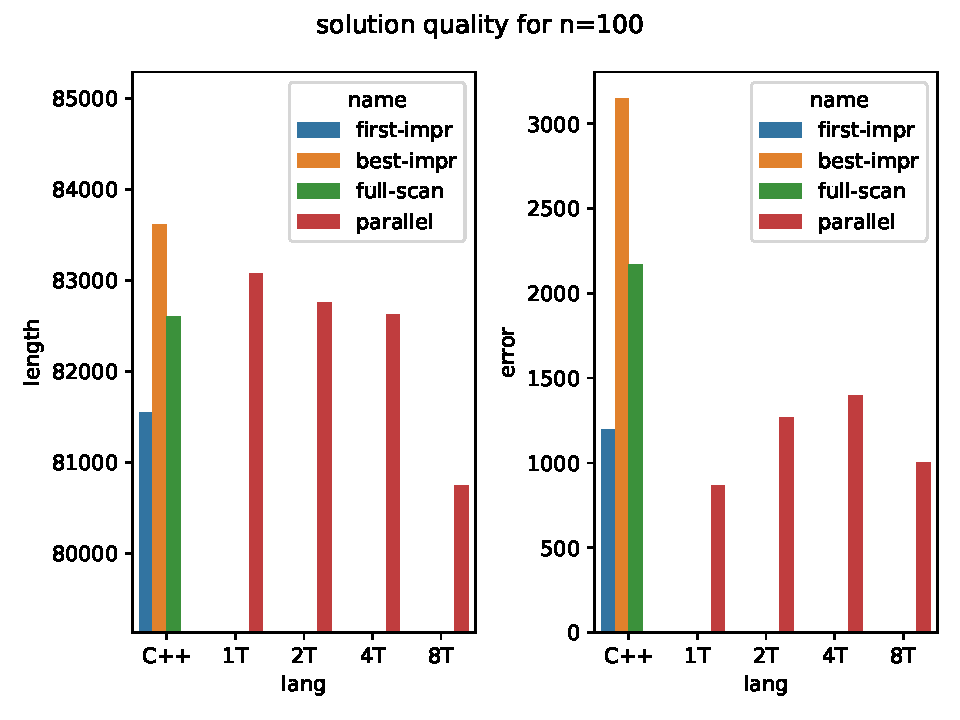
\includegraphics[keepaspectratio, height=0.9\textheight]{3_n100_solution_quality.pdf}
		
		\column{0.4\textwidth}
		\begin{itemize}
			\item idea: run fastest algo multiple times
			\item use randomness for (usually) good solutions
		\end{itemize}
	\end{columns}
\end{frame}

\begin{frame}[fragile]{3: twoopt + analysis [2]}
\begin{columns}[T]
	\column{0.6\textwidth}
	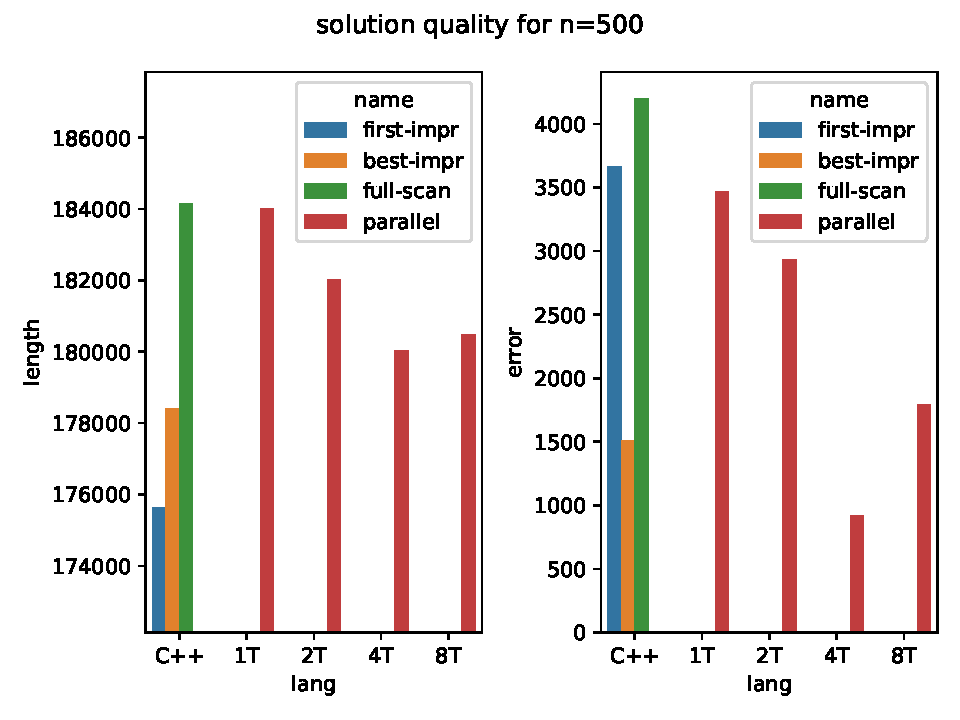
\includegraphics[keepaspectratio, height=0.9\textheight]{3_n500_solution_quality.pdf}
	
	\column{0.4\textwidth}
	\begin{itemize}
		\item idea: run fastest algo multiple times
		\item use randomness for (usually) good solutions
	\end{itemize}
\end{columns}
\end{frame}

\begin{frame}[fragile]{3: twoopt + analysis [2]}
	\begin{columns}[T]
		\column{0.6\textwidth}
		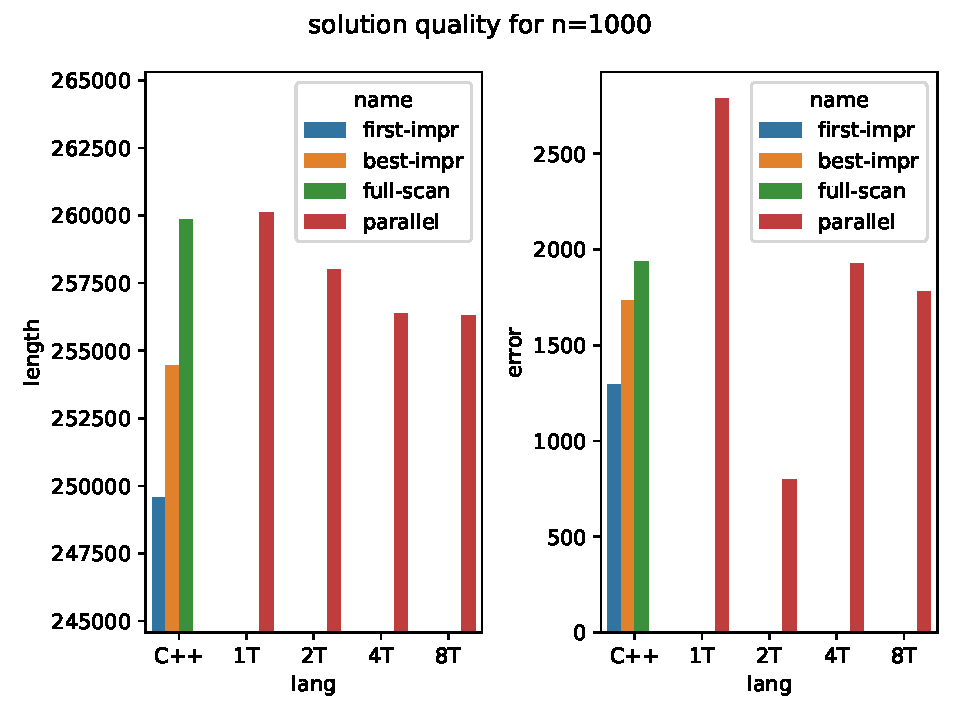
\includegraphics[keepaspectratio, height=0.9\textheight]{3_n1000_solution_quality.pdf}
		
		\column{0.4\textwidth}
		\begin{itemize}
			\item idea: run fastest algo multiple times
			\item use randomness for (usually) good solutions
			\item more threads = better solutions (usually)
			\item more threads = less deviation (usually)
		\end{itemize}
	\end{columns}
\end{frame}


\begin{frame}[fragile]{3: twoopt + analysis [3]}
	\begin{columns}[T]
		\column{0.6\textwidth}
		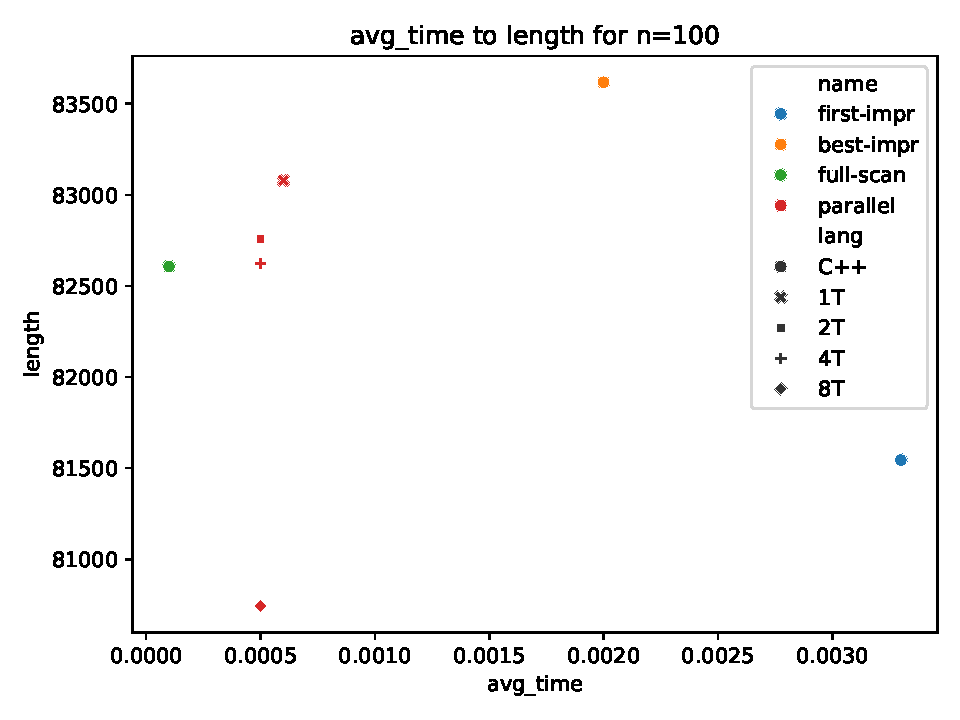
\includegraphics[keepaspectratio, height=0.9\textheight]{3_n100_time_length_parallel.pdf}
		
		\column{0.4\textwidth}
		\begin{itemize}
			\item slower than full-scan\\
				$\implies$ threading overhead
			\item faster than others
		\end{itemize}
	\end{columns}
\end{frame}

\begin{frame}[fragile]{3: twoopt + analysis [3]}
\begin{columns}[T]
	\column{0.6\textwidth}
	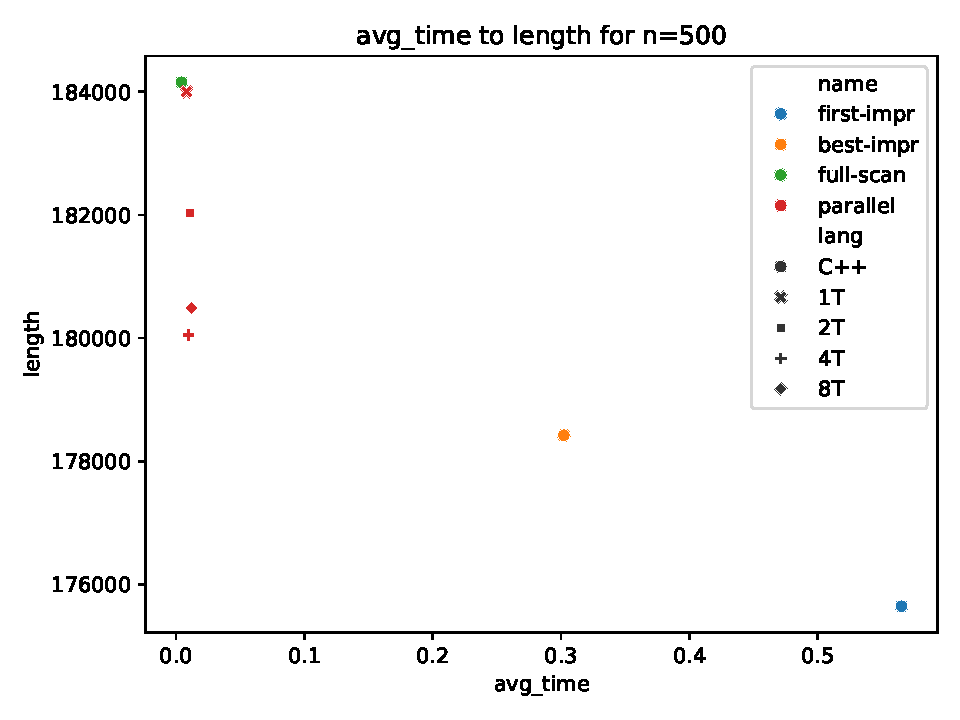
\includegraphics[keepaspectratio, height=0.9\textheight]{3_n500_time_length_parallel.pdf}
	
	\column{0.4\textwidth}
	\begin{itemize}
		\item slower than full-scan\\
		$\implies$ threading overhead
		\item faster than others
		\item threading overhead fades with higher $n$
	\end{itemize}
\end{columns}
\end{frame}

\begin{frame}[fragile]{3: twoopt + analysis [3]}
	\begin{columns}[T]
		\column{0.6\textwidth}
		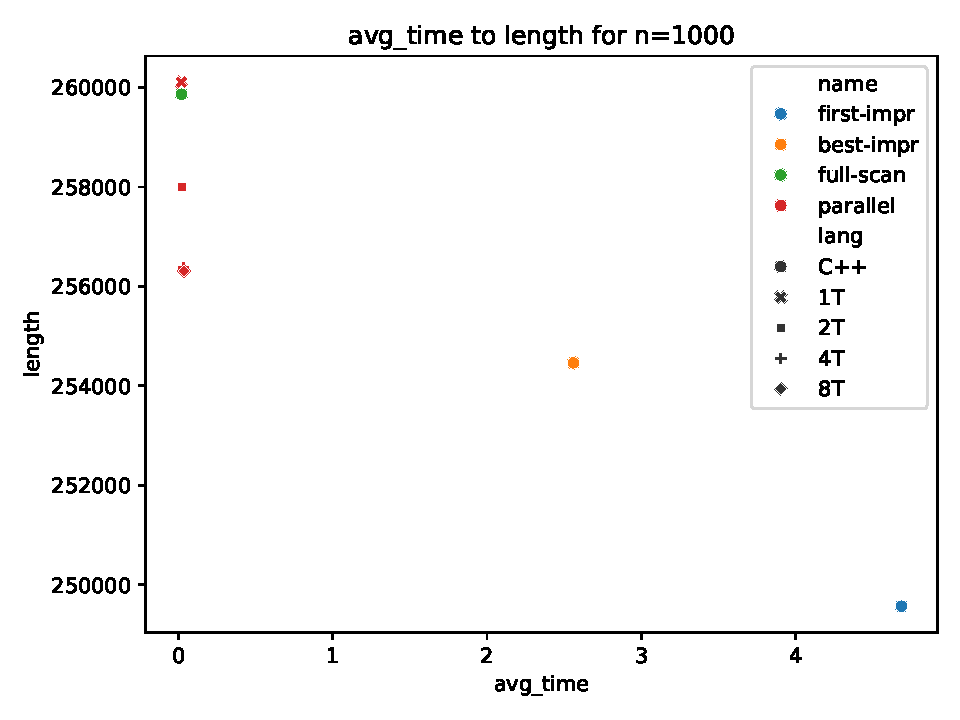
\includegraphics[keepaspectratio, height=0.9\textheight]{3_n1000_time_length_parallel.pdf}
		
		\column{0.4\textwidth}
		\begin{itemize}
			\item slower than full-scan\\
			$\implies$ threading overhead
			\item faster than others
			\item threading overhead fades with higher $n$
			\item solution quality improved
		\end{itemize}
	\end{columns}
\end{frame}
\begin{frame}[fragile]{3: twoopt + analysis [3]}
	\begin{columns}[T]
		\column{0.6\textwidth}
		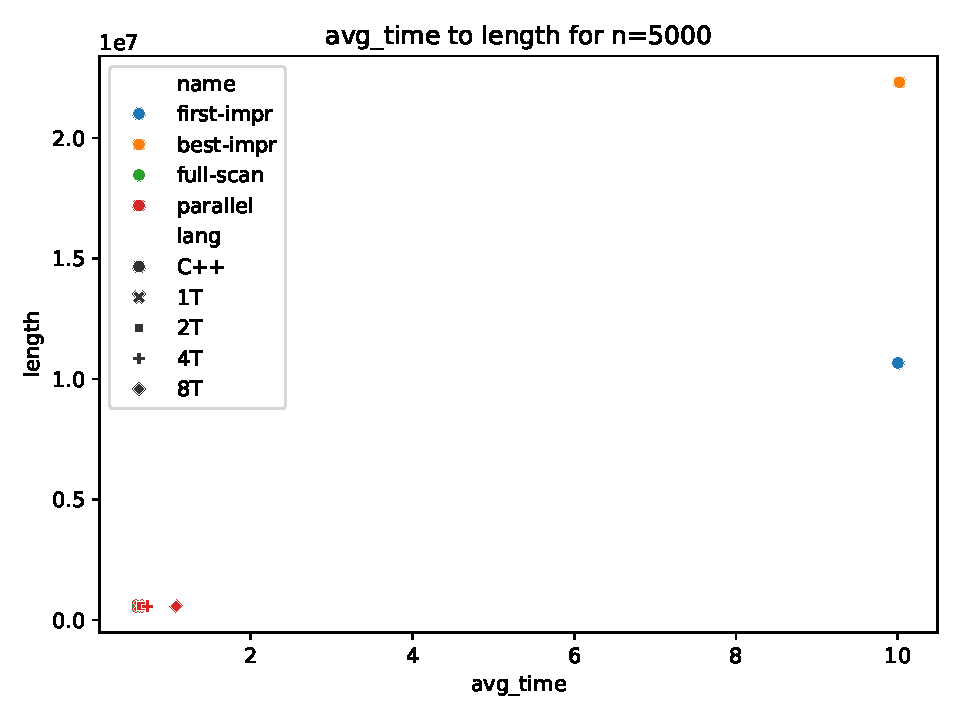
\includegraphics[keepaspectratio, height=0.9\textheight]{3_n5000_time_length_parallel.pdf}
		
		\column{0.4\textwidth}
		\begin{itemize}
			\item slower than full-scan\\
			$\implies$ threading overhead
			\item faster than others
			\item threading overhead fades with higher $n$
			\item solution quality improved
		\end{itemize}
	\end{columns}
\end{frame}

\begin{frame}[fragile]{3: twoopt + analysis [3]}
	\begin{columns}[T]
		\column{0.6\textwidth}
		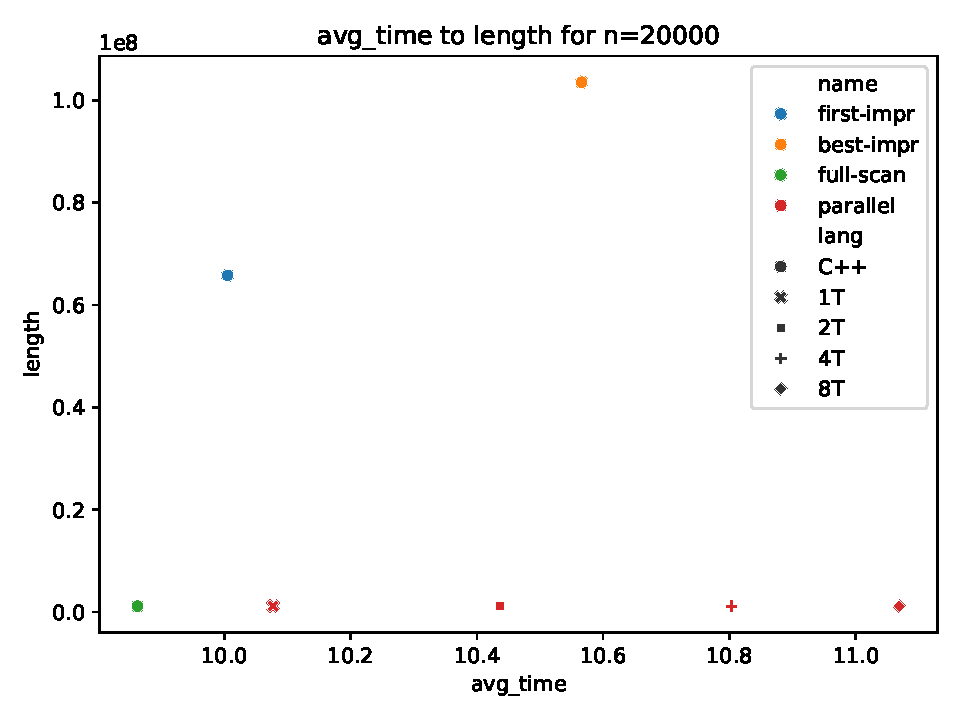
\includegraphics[keepaspectratio, height=0.9\textheight]{3_n20000_time_length_parallel.pdf}
		
		\column{0.4\textwidth}
		\begin{itemize}
			\item slower than full-scan\\
			$\implies$ threading overhead
			\item faster than others
			\item threading overhead fades with higher $n$
			\item solution quality improved...
			\item ... unless in timeout
		\end{itemize}
	\end{columns}
\end{frame}
\end{document}


